\part{Counting}
\section{Handout 02: Pigeonhole Principle, Permutations and Combinations}

\subsection{Overview}

This handout continues Part~I on counting. The main themes are:
\begin{itemize}[leftmargin=*]
    \item the pigeonhole principle and its generalized form;
    \item permutations and $r$-permutations as \emph{ordered} selections;
    \item combinations as \emph{unordered} selections;
    \item the relation
    \[
    P(n,r)=\binom{n}{r}r!;
    \]
    \item combinatorial proof, where one proves an identity by counting the same set in two different ways.
\end{itemize}

The central revision goal is to distinguish carefully between three recurring operations:
\[
\text{force existence},\qquad \text{choose and order},\qquad \text{choose without order}.
\]

\begin{examtip}[title={Main recognition goals for this handout}]
A typical question in this handout usually asks for one of the following:
\begin{enumerate}[leftmargin=*]
    \item prove that a repetition or collision \emph{must} occur;
    \item count ordered arrangements of distinct objects;
    \item count unordered selections;
    \item relate two counting expressions by interpreting them as counts of the same set.
\end{enumerate}
Before calculating, decide which of these four tasks you are facing.
\end{examtip}

%==================================================
\subsection{The Pigeonhole Principle}
%==================================================

The pigeonhole principle is a forcing statement: if too many objects are distributed among too few boxes, then some box must contain multiple objects. The principle is elementary, but its power lies in choosing the \emph{right} objects and the \emph{right} boxes.

\begin{theorem}{Pigeonhole Principle}{php-basic}
Let $k$ be a positive integer. If $k+1$ or more objects are placed into $k$ boxes, then at least one box contains at least two objects.
\end{theorem}

\begin{proof}
We prove the contrapositive. Suppose no box contains more than one object. Then each of the $k$ boxes contains at most one object, so the total number of objects is at most $k$. Therefore it is impossible to place $k+1$ or more objects into the $k$ boxes under this assumption. Hence, if $k+1$ or more objects are placed into $k$ boxes, some box must contain at least two objects.
\end{proof}

\begin{keyformula}[title={Most basic forcing pattern}]
\[
\text{If } \#\text{objects}>\#\text{boxes}, \text{ then some box contains at least two objects.}
\]
\end{keyformula}

\begin{examplebox}[title={Tutorial 2, Question 1}]
Show that if there are $30$ students in a class, then at least two have last names beginning with the same letter.

\textbf{Solution.}
Let the objects be the $30$ students. Let the boxes be the $26$ letters of the English alphabet. Each student is assigned to the box determined by the first letter of the student's last name. Since
\[
30>26,
\]
the pigeonhole principle shows that at least two students must be assigned to the same box. Hence at least two students have last names beginning with the same letter.
\end{examplebox}

\begin{commonmistake}[title={Choosing the wrong boxes}]
In pigeonhole arguments, the main difficulty is usually not the theorem itself but the modelling. The ``boxes'' are the categories into which the objects are classified. A weak or unnatural choice of boxes can make the principle useless.
\end{commonmistake}

\subsubsection{Floor and ceiling}

The generalized pigeonhole principle is most naturally written using the ceiling function.

\begin{definition}{Floor and ceiling}{floor-ceiling}
For a real number $x$:
\begin{itemize}[leftmargin=*]
    \item the \emph{floor} of $x$, denoted $\lfloor x\rfloor$, is the unique integer $n$ such that
    \[
    n\le x<n+1;
    \]
    \item the \emph{ceiling} of $x$, denoted $\lceil x\rceil$, is the unique integer $n$ such that
    \[
    n-1<x\le n.
    \]
\end{itemize}
\end{definition}

\begin{theorem}{Generalized Pigeonhole Principle}{php-general}
If $N$ objects are placed into $k$ boxes, then at least one box contains at least
\[
\left\lceil \frac{N}{k}\right\rceil
\]
objects.
\end{theorem}

\begin{proof}
Suppose no box contains as many as $\lceil N/k\rceil$ objects. Then every box contains at most
\[
\left\lceil \frac{N}{k}\right\rceil-1
\]
objects. Hence the total number of objects is at most
\[
k\left(\left\lceil \frac{N}{k}\right\rceil-1\right).
\]
Since $\lceil N/k\rceil < N/k+1$, we obtain
\[
k\left(\left\lceil \frac{N}{k}\right\rceil-1\right)<k\left(\frac{N}{k}+1-1\right)=N,
\]
which contradicts the existence of $N$ objects. Therefore some box contains at least $\lceil N/k\rceil$ objects.
\end{proof}

\begin{keyformula}[title={Generalized form}]
\[
\text{maximum box occupancy}\ge \left\lceil\frac{N}{k}\right\rceil.
\]
\end{keyformula}

\begin{extension}[title={Average-value viewpoint}]
The quantity $N/k$ is the average number of objects per box. The generalized pigeonhole principle says that the most occupied box cannot lie below the average; in integer form, it must contain at least
\[
\left\lceil \frac{N}{k}\right\rceil
\]
objects. This is often the fastest way to interpret the theorem in exam questions.
\end{extension}

\begin{examplebox}[title={Hair coincidence}]
Suppose Singapore has more than $5{,}000{,}000$ non-bald people, and assume each person has fewer than $200{,}000$ hairs on their head. Show that there exist $26$ people with the same number of hairs.

\textbf{Solution.}
Let the objects be the non-bald people, so $N\ge 5{,}000{,}001$. Let the boxes be the possible hair counts $1,2,\dots,199{,}999$, so $k\le 199{,}999$. By the generalized pigeonhole principle, some hair count occurs at least
\[
\left\lceil \frac{5{,}000{,}001}{199{,}999}\right\rceil=26
\]
times.
\end{examplebox}

\begin{examplebox}[title={Tutorial 2, Question 2}]
$250$ courses have their final examinations scheduled over $20$ days. There are $3$ time slots per day, and at most two exams can take place in the same venue at the same time. Show that at least $3$ venues are needed.

\textbf{Solution.}
There are
\[
20\cdot 3=60
\]
distinct time slots. A single venue can host at most $2$ exams per time slot, so one venue can host at most
\[
60\cdot 2=120
\]
exams. Hence two venues can host at most
\[
2\cdot 120=240
\]
exams, which is less than $250$. Therefore two venues do not suffice, so at least $3$ venues are required.
\end{examplebox}

\begin{examplebox}[title={A multiple of $n$ using only digits $0$ and $1$}]
Show that for every positive integer $n$, there exists a multiple of $n$ whose decimal expansion uses only the digits $0$ and $1$.

\textbf{Solution.}
Consider the $n+1$ integers
\[
1,\ 11,\ 111,\ \dots,\ \underbrace{11\cdots 1}_{n+1\text{ ones}}.
\]
When divided by $n$, these integers produce only $n$ possible remainders. Hence, by the pigeonhole principle, two of them have the same remainder modulo $n$. Let these be $x$ and $y$ with $x>y$. Then $x-y$ is divisible by $n$. Also, subtracting a shorter repunit from a longer one produces a decimal number consisting only of $1$'s followed by $0$'s, so $x-y$ uses only the digits $0$ and $1$.
\end{examplebox}

\begin{extension}[title={How to search for the right pigeonhole model}]
A productive template is:
\begin{enumerate}[leftmargin=*]
    \item decide what the objects are;
    \item classify each object by a feature that takes only a limited number of values;
    \item use those feature-values as the boxes.
\end{enumerate}
For remainders, initials, hair counts, weekdays, parity classes, and residue classes, this often gives the correct formulation immediately.
\end{extension}

%==================================================
\subsection{Permutations}
%==================================================

Permutations count \emph{ordered} selections. The selected elements matter, and the order in which they appear also matters.

\begin{definition}{Permutation and $r$-permutation}{perm-rperm}
Let $S$ be a finite set of distinct elements.
\begin{itemize}[leftmargin=*]
    \item A \emph{permutation} of $S$ is an ordered arrangement of all elements of $S$.
    \item If $|S|=n$ and $0\le r\le n$, an \emph{$r$-permutation} of $S$ is an ordered selection of $r$ distinct elements from $S$.
\end{itemize}
The number of $r$-permutations of an $n$-element set is denoted by $P(n,r)$.
\end{definition}

\begin{theorem}{Formula for $P(n,r)$}{perm-formula}
For integers $n$ and $r$ with $1\le r\le n$,
\[
P(n,r)=n(n-1)(n-2)\cdots (n-r+1).
\]
Equivalently,
\[
P(n,r)=\frac{n!}{(n-r)!}.
\]
\end{theorem}

\begin{proof}
To form an $r$-permutation, choose the first entry in $n$ ways, the second in $n-1$ ways, and continue until the $r$-th entry, which can be chosen in
\[
n-(r-1)=n-r+1
\]
ways. By the product rule,
\[
P(n,r)=n(n-1)\cdots(n-r+1).
\]
Since
\[
n!=n(n-1)\cdots(n-r+1)(n-r)!,
\]
dividing by $(n-r)!$ gives the factorial form.
\end{proof}

\begin{keyformula}[title={$r$-permutations}]
\[
P(n,r)=n(n-1)\cdots(n-r+1)=\frac{n!}{(n-r)!}.
\]
Special cases:
\[
P(n,n)=n!,\qquad P(n,1)=n,\qquad P(n,0)=1.
\]
\end{keyformula}

\begin{examplebox}[title={COMPUTER}]
How many ways can the letters in the word \texttt{COMPUTER} be arranged in a row?

\textbf{Solution.}
The word contains $8$ distinct letters. Hence the number of arrangements is
\[
P(8,8)=8!=40{,}320.
\]
\end{examplebox}

\begin{examplebox}[title={COMPUTER with a block constraint}]
How many arrangements of the letters in \texttt{COMPUTER} have the letters \texttt{CO} next to each other in that order?

\textbf{Solution.}
Treat \texttt{CO} as one block. Then the objects being arranged are
\[
\texttt{CO},\ \texttt{M},\ \texttt{P},\ \texttt{U},\ \texttt{T},\ \texttt{E},\ \texttt{R},
\]
so there are $7$ distinct objects. Hence the number of such arrangements is
\[
7!=5{,}040.
\]
\end{examplebox}

\begin{examplebox}[title={Prize winners}]
How many ways are there to select a first-prize winner, a second-prize winner, and a third-prize winner from $200$ students?

\textbf{Solution.}
This is an ordered selection of $3$ distinct students from $200$, so the answer is
\[
P(200,3)=200\cdot 199\cdot 198=7{,}880{,}400.
\]
\end{examplebox}

\begin{commonmistake}[title={Confusing selection with ordering}]
The expressions ``choose $r$ objects'' and ``arrange $r$ objects'' describe different tasks. If the roles are \emph{first prize, second prize, third prize}, then order matters. If the task is simply to form a committee, order does not matter.
\end{commonmistake}

\begin{extension}[title={Block method as a structural permutation trick}]
Whenever several objects are required to stay together in a fixed internal order, treat them as a single super-object. If the internal order is not fixed, first count the arrangements of the block as a unit and then multiply by the number of internal arrangements.
\end{extension}

%==================================================
\subsection{Combinations}
%==================================================

Combinations count \emph{unordered} selections. Only the chosen elements matter; the order in which they are listed does not.

\begin{definition}{$r$-combination}{combination-def}
Let $S$ be a set with $n$ elements. An \emph{$r$-combination} of $S$ is an unordered selection of $r$ elements from $S$, where $0\le r\le n$.

The number of $r$-combinations of an $n$-element set is denoted by
\[
C(n,r)\qquad\text{or}\qquad \binom{n}{r}.
\]
\end{definition}

\begin{examplebox}[title={A first example}]
Let $S=\{a,b,c\}$. The $2$-combinations are
\[
\{a,b\},\ \{a,c\},\ \{b,c\}.
\]
Hence
\[
C(3,2)=3.
\]
Note that $\{a,b\}$ and $\{b,a\}$ are the same combination.
\end{examplebox}

\subsubsection{Relation between permutations and combinations}

The key observation is that an ordered selection may be built in two stages:
\begin{enumerate}[leftmargin=*]
    \item choose the $r$ elements;
    \item order the chosen $r$ elements.
\end{enumerate}

% Choose-then-order diagram illustrating P(n,r)=C(n,r)r!
\begin{center}
\begin{tikzpicture}[>=stealth, node distance=2.8cm]
    \node[draw, rounded corners, align=center, inner sep=6pt] (A) {choose an $r$-subset\\$\binom{n}{r}$ ways};
    \node[draw, rounded corners, align=center, inner sep=6pt, right of=A, xshift=1.2cm] (B) {order the chosen elements\\$r!$ ways};
    \node[draw, rounded corners, align=center, inner sep=6pt, right of=B, xshift=1.2cm] (C) {obtain an\\$r$-permutation};
    \draw[->, thick] (A) -- (B);
    \draw[->, thick] (B) -- (C);
\end{tikzpicture}
\end{center}

\begin{theorem}{Formula for combinations}{comb-formula}
For integers $n$ and $r$ with $0\le r\le n$,
\[
\binom{n}{r}=\frac{n!}{r!(n-r)!}.
\]
Equivalently,
\[
P(n,r)=\binom{n}{r}r!.
\]
\end{theorem}

\begin{proof}
Every $r$-permutation is obtained by first choosing an $r$-element subset and then ordering its $r$ elements. There are $\binom{n}{r}$ ways to choose the subset and $r!$ ways to order it. Hence
\[
P(n,r)=\binom{n}{r}r!.
\]
Using
\[
P(n,r)=\frac{n!}{(n-r)!},
\]
we obtain
\[
\binom{n}{r}=\frac{P(n,r)}{r!}=\frac{n!}{r!(n-r)!}.
\]
\end{proof}

\begin{keyformula}[title={Binomial coefficient formula}]
\[
\binom{n}{r}=\frac{n!}{r!(n-r)!}.
\]
Special cases:
\[
\binom{n}{0}=1,\qquad \binom{n}{1}=n,\qquad \binom{n}{n-1}=n,\qquad \binom{n}{n}=1.
\]
\end{keyformula}

\begin{extension}[title={Canonical choose-then-order decomposition}]
The identity
\[
P(n,r)=\binom{n}{r}r!
\]
is not just a formula. It describes the exact structure of an ordered selection: first determine \emph{which} elements appear, then determine \emph{in what order} they appear. This structural viewpoint is often more useful than memorising the factorial form directly.
\end{extension}

\begin{examplebox}[title={Bit strings with exactly $r$ ones}]
How many $0$-$1$ strings of length $n$ contain exactly $r$ ones?

\textbf{Solution.}
Such a string is completely determined by the positions of the $r$ ones. Hence we choose $r$ positions from the $n$ available positions, giving
\[
\binom{n}{r}
\]
strings.
\end{examplebox}

\begin{examplebox}[title={Selecting a team}]
There are $9$ boys and $11$ girls. How many ways are there to choose $3$ boys and $4$ girls to form a team?

\textbf{Solution.}
Choose the boys and girls independently:
\[
\binom{9}{3}\binom{11}{4}=84\cdot 330=27{,}720.
\]
\end{examplebox}

\begin{examplebox}[title={A required pair}]
Suppose two members $A$ and $B$ of a group of $12$ insist on working as a pair: any $5$-person team must contain either both or neither. How many such teams are possible?

\textbf{Solution.}
There are two disjoint cases.
\begin{itemize}[leftmargin=*]
    \item Both $A$ and $B$ are included: choose the remaining $3$ members from the other $10$, giving $\binom{10}{3}$ teams.
    \item Neither $A$ nor $B$ is included: choose all $5$ members from the other $10$, giving $\binom{10}{5}$ teams.
\end{itemize}
Therefore the total number is
\[
\binom{10}{3}+\binom{10}{5}=120+252=372.
\]
\end{examplebox}

\begin{examplebox}[title={Powerball}]
In Powerball, five regular numbers are chosen from $1$ to $69$, and one special Powerball number is chosen from $1$ to $26$. How many tickets are possible?

\textbf{Solution.}
The five regular numbers form an unordered selection of $5$ distinct integers from $69$, so there are $\binom{69}{5}$ possibilities. The Powerball is then chosen in $26$ ways. Hence the total number of tickets is
\[
\binom{69}{5}\cdot 26=292{,}201{,}338.
\]
\end{examplebox}

\begin{examplebox}[title={Poker hands}]
How many $5$-card poker hands can be dealt from a standard deck of $52$ cards?

\textbf{Solution.}
A hand is an unordered selection of $5$ cards from $52$, so the number of hands is
\[
\binom{52}{5}=2{,}598{,}960.
\]
\end{examplebox}

\subsubsection{Symmetry of binomial coefficients}

\begin{theorem}{Symmetry identity}{comb-symmetry}
For integers $n$ and $r$ with $0\le r\le n$,
\[
\binom{n}{r}=\binom{n}{n-r}.
\]
\end{theorem}

\begin{proof}
Using the factorial formula,
\[
\binom{n}{r}=\frac{n!}{r!(n-r)!}=\frac{n!}{(n-r)![n-(n-r)]!}=\binom{n}{n-r}.
\]
\end{proof}

\begin{extension}[title={Combinatorial meaning of the symmetry}]
Choosing $r$ objects to include is equivalent to choosing the $n-r$ objects to exclude. This gives a direct bijection between $r$-subsets and $(n-r)$-subsets: send each subset to its complement.
\end{extension}

\begin{commonmistake}[title={Combination formulas are for unordered selections only}]
A formula such as $\binom{n}{r}$ should not be used unless different orderings of the same chosen elements represent the \emph{same} object. Cards in a hand form a combination; prize winners with distinct ranks form a permutation.
\end{commonmistake}

%==================================================
\subsection{Combinatorial Proof}
%==================================================

\begin{definition}{Combinatorial proof}{comb-proof}
A \emph{combinatorial proof} of an identity is a proof that interprets both sides of the identity as counting the same set of objects in two different ways.
\end{definition}

The point is not algebraic manipulation. Instead, one identifies one collection of objects and counts it by two valid descriptions.

\begin{examplebox}[title={Pascal identity}]
Prove that for integers $n\ge k\ge 1$,
\[
\binom{n}{k}=\binom{n-1}{k}+\binom{n-1}{k-1}.
\]

\textbf{Combinatorial proof.}
Count the number of $k$-element subsets of an $n$-element set containing a distinguished element $x$ or not containing $x$.

Let the ground set be
\[
S=\{x\}\cup T,
\qquad |T|=n-1.
\]
The left-hand side counts all $k$-element subsets of $S$, so it equals $\binom{n}{k}$.

Now partition these subsets into two disjoint classes:
\begin{itemize}[leftmargin=*]
    \item subsets not containing $x$: choose all $k$ elements from $T$, giving $\binom{n-1}{k}$ choices;
    \item subsets containing $x$: then the remaining $k-1$ elements are chosen from $T$, giving $\binom{n-1}{k-1}$ choices.
\end{itemize}
Adding the disjoint cases gives
\[
\binom{n}{k}=\binom{n-1}{k}+\binom{n-1}{k-1}.
\]
\end{examplebox}

\begin{examplebox}[title={An equality of two partition counts}]
Show that the number of ways to write
\[
n=a+b
\qquad\text{with}\qquad a\ge b\ge 0
\]
is equal to the number of ways to write
\[
n=c+2d
\qquad\text{with}\qquad c,d\ge 0.
\]

\textbf{Combinatorial proof.}
Given a representation $n=a+b$ with $a\ge b\ge 0$, define
\[
c=a-b,\qquad d=b.
\]
Then
\[
c+2d=(a-b)+2b=a+b=n,
\]
and $c,d\ge 0$. Conversely, given $n=c+2d$ with $c,d\ge 0$, set
\[
a=c+d,\qquad b=d.
\]
Then
\[
a+b=(c+d)+d=c+2d=n,
\qquad a\ge b\ge 0.
\]
These constructions are inverse to each other, so they define a bijection between the two families of representations. Therefore the two counts are equal.
\end{examplebox}

\begin{extension}[title={How to invent a combinatorial proof}]
A useful template is:
\begin{enumerate}[leftmargin=*]
    \item decide what set of objects one side is naturally counting;
    \item check whether the other side counts the same set after partitioning, reordering, or re-encoding the objects;
    \item make the two counting viewpoints explicit.
\end{enumerate}
In many binomial identities, the right side arises by partitioning the same family into disjoint cases.
\end{extension}

%==================================================
\subsection{Special Techniques}
%==================================================

\subsubsection*{1. Worst-case construction for pigeonhole problems}
To determine the smallest number that guarantees a repetition or threshold occupancy, first maximise how many objects can be placed while still \emph{avoiding} the desired conclusion. Then add one more object.

\subsubsection*{2. Average-occupancy interpretation}
When using the generalized pigeonhole principle, compute
\[
\left\lceil \frac{N}{k}\right\rceil
\]
and interpret it as the minimum guaranteed size of the most populated box.

\subsubsection*{3. Choose-then-order}
To count ordered selections, it is often efficient to first choose the participating elements and then order them:
\[
P(n,r)=\binom{n}{r}r!.
\]
This is especially useful when a question mixes unordered selection with labelled roles.

\subsubsection*{4. Block method in permutations}
When specified objects must stay together, compress them into a single block. If the internal order is flexible, multiply by the number of internal block arrangements afterward.

\subsubsection*{5. Convert exact-content questions into position choices}
Questions such as ``exactly $r$ ones'' are often best solved by choosing positions rather than building strings directly.

\subsubsection*{6. Prove identities by counting one set in two ways}
For combinatorial proof, do not start with algebra. Start by asking: \emph{what family of objects could both sides be counting?}

\begin{examtip}[title={High-yield diagnostic checklist}]
Before finalising a solution from this handout, verify:
\begin{enumerate}[leftmargin=*]
    \item Have I identified the boxes correctly in the pigeonhole model?
    \item Have I decided correctly whether order matters?
    \item If I used $\binom{n}{r}$, did I justify why the selection is unordered?
    \item If I used $P(n,r)$, did I account for distinct roles or positions?
    \item If I wrote a combinatorial proof, did both sides count the same set of objects?
\end{enumerate}
\end{examtip}

%==================================================
\subsection{Summary Table}
%==================================================

\begin{center}
\small
\begin{tabular}{@{}p{0.25\textwidth}p{0.25\textwidth}p{0.38\textwidth}@{}}
\toprule
\textbf{Problem type} & \textbf{Main tool} & \textbf{Typical signal} \\
\midrule
forced repetition / collision & pigeonhole principle & more objects than categories \\
minimum guaranteed occupancy & generalized pigeonhole principle & distribute $N$ objects among $k$ boxes \\
ordered selection of $r$ distinct objects & $P(n,r)$ & rank, arrange, first/second/third, line up \\
unordered selection of $r$ objects & $\binom{n}{r}$ & choose, committee, hand, team \\
identity of counting expressions & combinatorial proof & prove two formulas are equal by interpretation \\
\bottomrule
\end{tabular}
\end{center}

\begin{commonmistake}[title={Final distinction to remember}]
The expressions
\[
P(n,r),\qquad \binom{n}{r},\qquad \left\lceil\frac{N}{k}\right\rceil
\]
solve fundamentally different kinds of problems. A large fraction of exam errors in this handout come from selecting the correct formula too early, before deciding whether the problem is about forcing, ordering, or unordered choice.
\end{commonmistake}